% AttnLRP (Achtibat et al., 2024) relevance propagation through a multi-head
% attention block. Forward graph in black, backward relevance in red.
% Rules: epsilon-LRP on linear projections, uniform bilinear split on the two
% matmuls (half the relevance to each operand), Taylor rule through the softmax,
% exact reshape for head split/merge.
% Compile: pdflatex attnlrp_propagation.tex
\documentclass[tikz,border=10pt]{standalone}
\usepackage[T1]{fontenc}
\usepackage{helvet}
\usepackage{amsmath}
\renewcommand{\familydefault}{\sfdefault}
\usetikzlibrary{positioning,arrows.meta,calc,backgrounds,fit}

\definecolor{linC}{RGB}{31,78,145}
\definecolor{bilC}{RGB}{192,96,10}
\definecolor{gateC}{RGB}{122,44,140}
\definecolor{permC}{RGB}{34,110,50}
\definecolor{relC}{RGB}{176,20,30}

\begin{document}
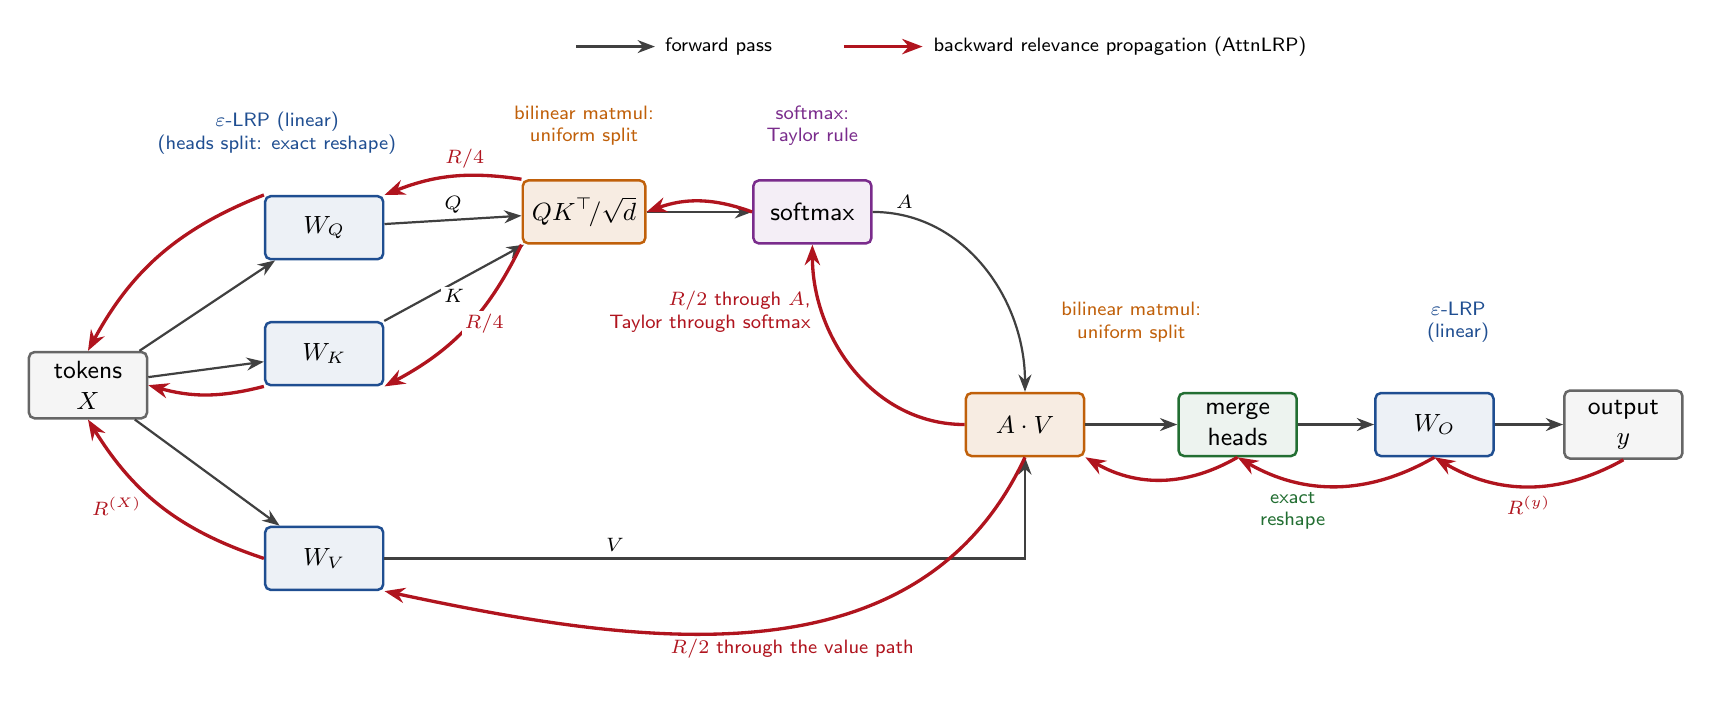
\begin{tikzpicture}[
  op/.style={draw, rounded corners=2pt, minimum height=8mm, minimum width=15mm,
             align=center, font=\small, line width=0.9pt, fill=white},
  lin/.style={op, draw=linC, fill=linC!8},
  bil/.style={op, draw=bilC, fill=bilC!12},
  gate/.style={op, draw=gateC, fill=gateC!8},
  perm/.style={op, draw=permC, fill=permC!8},
  io/.style={op, draw=black!60, fill=black!4},
  fwd/.style={-{Stealth[length=2.2mm]}, line width=0.8pt, draw=black!75},
  rel/.style={-{Stealth[length=2.6mm]}, line width=1.2pt, draw=relC},
  flab/.style={font=\scriptsize, fill=white, inner sep=1pt},
  rlab/.style={font=\scriptsize, text=relC, fill=white, inner sep=1pt},
  rul/.style={font=\scriptsize, align=center},
  leg/.style={font=\scriptsize, anchor=west},
]

% ---------------- forward pipeline ----------------
\node[io]   (x)  at (0.0,-0.4)  {tokens\\$X$};
\node[lin]  (wq) at (3.0, 1.6)  {$W_Q$};
\node[lin]  (wk) at (3.0, 0.0)  {$W_K$};
\node[lin]  (wv) at (3.0,-2.6)  {$W_V$};
\node[bil]  (qk) at (6.3, 1.8)  {$QK^{\top}\!/\sqrt{d}$};
\node[gate] (sm) at (9.2, 1.8)  {softmax};
\node[bil]  (av) at (11.9,-0.9) {$A \cdot V$};
\node[perm] (mh) at (14.6,-0.9) {merge\\heads};
\node[lin]  (wo) at (17.1,-0.9) {$W_O$};
\node[io]   (y)  at (19.5,-0.9) {output\\$y$};

\draw[fwd] (x) -- (wq);
\draw[fwd] (x) -- (wk);
\draw[fwd] (x) -- (wv);
\draw[fwd] (wq) -- node[flab, pos=0.5, above=1pt]{$Q$} (qk);
\draw[fwd] (wk) -- node[flab, pos=0.5, below=1pt]{$K$} (qk);
\draw[fwd] (qk) -- (sm);
\draw[fwd] (sm.east) to[out=0, in=90] node[flab, pos=0.12, above=1pt]{$A$} (av.north);
\draw[fwd] (wv.east) -| node[flab, pos=0.18, above=1pt]{$V$} (av.south);
\draw[fwd] (av) -- (mh);
\draw[fwd] (mh) -- (wo);
\draw[fwd] (wo) -- (y);

% ---------------- rule labels ----------------
\node[rul, text=linC]  at (2.4, 2.8)   {$\varepsilon$-LRP (linear)\\(heads split: exact reshape)};
\node[rul, text=bilC]  at (6.3, 2.9)   {bilinear matmul:\\uniform split};
\node[rul, text=gateC] at (9.2, 2.9)   {softmax:\\Taylor rule};
\node[rul, text=bilC]  at (13.25, 0.4) {bilinear matmul:\\uniform split};
\node[rul, text=permC] at (15.3, -2.0) {exact\\reshape};
\node[rul, text=linC]  at (17.4, 0.4)  {$\varepsilon$-LRP\\(linear)};

% ---------------- backward relevance ----------------
\draw[rel] (y.south) to[bend left=30] node[rlab, below=2pt]{$R^{(y)}$} (wo.south);
\draw[rel] (wo.south) to[bend left=30] (mh.south);
\draw[rel] (mh.south) to[bend left=30] (av.south east);

% value branch: half the relevance
\draw[rel] (av.south) to[out=-115, in=-12]
  node[rlab, pos=0.45, below=3pt]{$R/2$ through the value path}
  (wv.south east);
\draw[rel] (wv.west) to[bend left=20] node[rlab, pos=0.6, below left=0pt]{$R^{(X)}$} (x.south);

% attention branch: half the relevance, Taylor through the softmax
\draw[rel] (av.west) to[out=180, in=-90]
  node[rlab, pos=0.75, left=3pt, align=right]{$R/2$ through $A$,\\Taylor through softmax}
  (sm.south);
\draw[rel] (sm.west) to[bend right=20] (qk.east);
\draw[rel] (qk.north west) to[bend right=15] node[rlab, pos=0.4, above=1pt]{$R/4$} (wq.north east);
\draw[rel] (qk.south west) to[bend left=18] node[rlab, pos=0.35, below=1pt]{$R/4$} (wk.south east);
\draw[rel] (wq.north west) to[bend right=20] (x.north);
\draw[rel] (wk.south west) to[bend left=15] (x.east);

% ---------------- legend ----------------
\draw[fwd] (6.2, 3.9) -- (7.2, 3.9) node[leg]{forward pass};
\draw[rel] (9.6, 3.9) -- (10.6, 3.9) node[leg]{backward relevance propagation (AttnLRP)};

\end{tikzpicture}
\end{document}
